\chapter{Chapter II}

\begin{verse}
A Monk there was, a fayre for the maistrie,\\
An outrider that loved venerie;\\
A manly man, to be an Abbot able,\\
Full many a daintie horse had he in stable:\\
And whan he rode, men might his bridle hear\\
Gingeling in a whistling wind as clear,\\
And eke as loud, as doth the chapell bell,\\
There as this lord was keeper of the cell.\\!
\attrib{--Chaucer.}
\end{verse}

\lettrine{N}{otwithstanding} the occasional exhortation and chiding of
his companion,
the noise of the horsemen's feet continuing to approach, Wamba could not
be prevented from lingering occasionally on the road, upon every
pretence which occurred; now catching from the hazel a cluster of
half-ripe nuts, and now turning his head to leer after a cottage maiden
who crossed their path. The horsemen, therefore, soon overtook them on
the road.

Their numbers amounted to ten men, of whom the two who rode foremost
seemed to be persons of considerable importance, and the others their
attendants. It was not difficult to ascertain the condition and
character of one of these personages. He was obviously an ecclesiastic
of high rank; his dress was that of a Cistercian Monk, but composed of
materials much finer than those which the rule of that order admitted.
His mantle and hood were of the best Flanders cloth, and fell in ample,
and not ungraceful folds, around a handsome, though somewhat corpulent
person. His countenance bore as little the marks of self-denial, as his
habit indicated contempt of worldly splendour. His features might have
been called good, had there not lurked under the pent-house of his eye,
that sly epicurean twinkle which indicates the cautious voluptuary. In
other respects, his profession and situation had taught him a ready
command over his countenance, which he could contract at pleasure into
solemnity, although its natural expression was that of good-humoured
social indulgence. In defiance of conventual rules, and the edicts of
popes and councils, the sleeves of this dignitary were lined and turned
up with rich furs, his mantle secured at the throat with a golden clasp,
and the whole dress proper to his order as much refined upon and
ornamented, as that of a quaker beauty of the present day, who, while
she retains the garb and costume of her sect continues to give to its
simplicity, by the choice of materials and the mode of disposing them, a
certain air of coquettish attraction, savouring but too much of the
vanities of the world.

This worthy churchman rode upon a well-fed ambling mule, whose furniture
was highly decorated, and whose bridle, according to the fashion of the
day, was ornamented with silver bells. In his seat he had nothing of the
awkwardness of the convent, but displayed the easy and habitual grace of
a well-trained horseman. Indeed, it seemed that so humble a conveyance
as a mule, in however good case, and however well broken to a pleasant
and accommodating amble, was only used by the gallant monk for
travelling on the road. A lay brother, one of those who followed in the
train, had, for his use on other occasions, one of the most handsome
Spanish jennets ever bred at Andalusia, which merchants used at that
time to import, with great trouble and risk, for the use of persons of
wealth and distinction. The saddle and housings of this superb palfrey
were covered by a long foot-cloth, which reached nearly to the ground,
and on which were richly embroidered, mitres, crosses, and other
ecclesiastical emblems. Another lay brother led a sumpter mule, loaded
probably with his superior's baggage; and two monks of his own order, of
inferior station, rode together in the rear, laughing and conversing
with each other, without taking much notice of the other members of the
cavalcade.

The companion of the church dignitary was a man past forty, thin,
strong, tall, and muscular; an athletic figure, which long fatigue and
constant exercise seemed to have left none of the softer part of the
human form, having reduced the whole to brawn, bones, and sinews, which
had sustained a thousand toils, and were ready to dare a thousand more.
His head was covered with a scarlet cap, faced with fur--of that kind
which the French call ``mortier'', from its resemblance to the shape of
an inverted mortar. His countenance was therefore fully displayed, and
its expression was calculated to impress a degree of awe, if not of
fear, upon strangers. High features, naturally strong and powerfully
expressive, had been burnt almost into Negro blackness by constant
exposure to the tropical sun, and might, in their ordinary state, be
said to slumber after the storm of passion had passed away; but the
projection of the veins of the forehead, the readiness with which the
upper lip and its thick black moustaches quivered upon the slightest
emotion, plainly intimated that the tempest might be again and easily
awakened. His keen, piercing, dark eyes, told in every glance a history
of difficulties subdued, and dangers dared, and seemed to challenge
opposition to his wishes, for the pleasure of sweeping it from his road
by a determined exertion of courage and of will; a deep scar on his brow
gave additional sternness to his countenance, and a sinister expression
to one of his eyes, which had been slightly injured on the same
occasion, and of which the vision, though perfect, was in a slight and
partial degree distorted.

The upper dress of this personage resembled that of his companion in
shape, being a long monastic mantle; but the colour, being scarlet,
showed that he did not belong to any of the four regular orders of
monks. On the right shoulder of the mantle there was cut, in white
cloth, a cross of a peculiar form. This upper robe concealed what at
first view seemed rather inconsistent with its form, a shirt, namely, of
linked mail, with sleeves and gloves of the same, curiously plaited and
interwoven, as flexible to the body as those which are now wrought in
the stocking-loom, out of less obdurate materials. The fore-part of his
thighs, where the folds of his mantle permitted them to be seen, were
also covered with linked mail; the knees and feet were defended by
splints, or thin plates of steel, ingeniously jointed upon each other;
and mail hose, reaching from the ankle to the knee, effectually
protected the legs, and completed the rider's defensive armour. In his
girdle he wore a long and double-edged dagger, which was the only
offensive weapon about his person.

He rode, not a mule, like his companion, but a strong hackney for the
road, to save his gallant war-horse, which a squire led behind, fully
accoutred for battle, with a chamfron or plaited head-piece upon his
head, having a short spike projecting from the front. On one side of the
saddle hung a short battle-axe, richly inlaid with Damascene carving; on
the other the rider's plumed head-piece and hood of mail, with a long
two-handed sword, used by the chivalry of the period. A second squire
held aloft his master's lance, from the extremity of which fluttered a
small banderole, or streamer, bearing a cross of the same form with that
embroidered upon his cloak. He also carried his small triangular shield,
broad enough at the top to protect the breast, and from thence
diminishing to a point. It was covered with a scarlet cloth, which
prevented the device from being seen.

These two squires were followed by two attendants, whose dark visages,
white turbans, and the Oriental form of their garments, showed them to
be natives of some distant Eastern country.\footnote{Note B. Negro Slaves.
See page~\pageref{noteCII}.}

The whole appearance of this warrior and his retinue was wild and
outlandish; the dress of his squires was gorgeous, and his Eastern
attendants wore silver collars round their throats, and bracelets of the
same metal upon their swarthy arms and legs, of which the former were
naked from the elbow, and the latter from mid-leg to ankle. Silk and
embroidery distinguished their dresses, and marked the wealth and
importance of their master; forming, at the same time, a striking
contrast with the martial simplicity of his own attire. They were armed
with crooked sabres, having the hilt and baldric inlaid with gold, and
matched with Turkish daggers of yet more costly workmanship. Each of
them bore at his saddle-bow a bundle of darts or javelins, about four
feet in length, having sharp steel heads, a weapon much in use among the
Saracens, and of which the memory is yet preserved in the martial
exercise called ``El Jerrid'', still practised in the Eastern countries.

The steeds of these attendants were in appearance as foreign as their
riders. They were of Saracen origin, and consequently of Arabian
descent; and their fine slender limbs, small fetlocks, thin manes, and
easy springy motion, formed a marked contrast with the large-jointed,
heavy horses, of which the race was cultivated in Flanders and in
Normandy, for mounting the men-at-arms of the period in all the panoply
of plate and mail; and which, placed by the side of those Eastern
coursers, might have passed for a personification of substance and of
shadow.

The singular appearance of this cavalcade not only attracted the
curiosity of Wamba, but excited even that of his less volatile
companion. The monk he instantly knew to be the Prior of Jorvaulx Abbey,
well known for many miles around as a lover of the chase, of the
banquet, and, if fame did him not wrong, of other worldly pleasures
still more inconsistent with his monastic vows.

Yet so loose were the ideas of the times respecting the conduct of the
clergy, whether secular or regular, that the Prior Aymer maintained a
fair character in the neighbourhood of his abbey. His free and jovial
temper, and the readiness with which he granted absolution from all
ordinary delinquencies, rendered him a favourite among the nobility and
principal gentry, to several of whom he was allied by birth, being of a
distinguished Norman family. The ladies, in particular, were not
disposed to scan too nicely the morals of a man who was a professed
admirer of their sex, and who possessed many means of dispelling the
ennui which was too apt to intrude upon the halls and bowers of an
ancient feudal castle. The Prior mingled in the sports of the field with
more than due eagerness, and was allowed to possess the best-trained
hawks, and the fleetest greyhounds in the North Riding; circumstances
which strongly recommended him to the youthful gentry. With the old, he
had another part to play, which, when needful, he could sustain with
great decorum. His knowledge of books, however superficial, was
sufficient to impress upon their ignorance respect for his supposed
learning; and the gravity of his deportment and language, with the high
tone which he exerted in setting forth the authority of the church and
of the priesthood, impressed them no less with an opinion of his
sanctity. Even the common people, the severest critics of the conduct of
their betters, had commiseration with the follies of Prior Aymer. He was
generous; and charity, as it is well known, covereth a multitude of
sins, in another sense than that in which it is said to do so in
Scripture. The revenues of the monastery, of which a large part was at
his disposal, while they gave him the means of supplying his own very
considerable expenses, afforded also those largesses which he bestowed
among the peasantry, and with which he frequently relieved the
distresses of the oppressed. If Prior Aymer rode hard in the chase, or
remained long at the banquet,--if Prior Aymer was seen, at the early
peep of dawn, to enter the postern of the abbey, as he glided home from
some rendezvous which had occupied the hours of darkness, men only
shrugged up their shoulders, and reconciled themselves to his
irregularities, by recollecting that the same were practised by many of
his brethren who had no redeeming qualities whatsoever to atone for
them. Prior Aymer, therefore, and his character, were well known to our
Saxon serfs, who made their rude obeisance, and received his
``benedicite, mes filz,'' in return.

But the singular appearance of his companion and his attendants,
arrested their attention and excited their wonder, and they could
scarcely attend to the Prior of Jorvaulx' question, when he demanded if
they knew of any place of harbourage in the vicinity; so much were they
surprised at the half monastic, half military appearance of the swarthy
stranger, and at the uncouth dress and arms of his Eastern attendants.
It is probable, too, that the language in which the benediction was
conferred, and the information asked, sounded ungracious, though not
probably unintelligible, in the ears of the Saxon peasants.

``I asked you, my children,'' said the Prior, raising his voice, and
using the lingua Franca, or mixed language, in which the Norman and
Saxon races conversed with each other, ``if there be in this
neighbourhood any good man, who, for the love of God, and devotion to
Mother Church, will give two of her humblest servants, with their train,
a night's hospitality and refreshment?''

This he spoke with a tone of conscious importance, which formed a strong
contrast to the modest terms which he thought it proper to employ.

``Two of the humblest servants of Mother Church!'' repeated Wamba to
himself,--but, fool as he was, taking care not to make his observation
audible; ``I should like to see her seneschals, her chief butlers, and
other principal domestics!''

After this internal commentary on the Prior's speech, he raised his
eyes, and replied to the question which had been put.

``If the reverend fathers,'' he said, ``loved good cheer and soft
lodging, few miles of riding would carry them to the Priory of
Brinxworth, where their quality could not but secure them the most
honourable reception; or if they preferred spending a penitential
evening, they might turn down yonder wild glade, which would bring them
to the hermitage of Copmanhurst, where a pious anchoret would make them
sharers for the night of the shelter of his roof and the benefit of his
prayers.''

The Prior shook his head at both proposals.

``Mine honest friend,'' said he, ``if the jangling of thy bells had not
dizzied thine understanding, thou mightst know ``Clericus clericum non
decimat''; that is to say, we churchmen do not exhaust each other's
hospitality, but rather require that of the laity, giving them thus an
opportunity to serve God in honouring and relieving his appointed
servants.''

``It is true,'' replied Wamba, ``that I, being but an ass, am,
nevertheless, honoured to hear the bells as well as your reverence's
mule; notwithstanding, I did conceive that the charity of Mother Church
and her servants might be said, with other charity, to begin at home.''

``A truce to thine insolence, fellow,'' said the armed rider, breaking
in on his prattle with a high and stern voice, ``and tell us, if thou
canst, the road to--How call'd you your Franklin, Prior Aymer?''

``Cedric,'' answered the Prior; ``Cedric the Saxon.--Tell me, good
fellow, are we near his dwelling, and can you show us the road?''

``The road will be uneasy to find,'' answered Gurth, who broke silence
for the first time, ``and the family of Cedric retire early to rest.''

``Tush, tell not me, fellow,'' said the military rider; ``'tis easy for
them to arise and supply the wants of travellers such as we are, who
will not stoop to beg the hospitality which we have a right to
command.''

``I know not,'' said Gurth, sullenly, ``if I should show the way to my
master's house, to those who demand as a right, the shelter which most
are fain to ask as a favour.''

``Do you dispute with me, slave!'' said the soldier; and, setting spurs
to his horse, he caused him make a demivolte across the path, raising at
the same time the riding rod which he held in his hand, with a purpose
of chastising what he considered as the insolence of the peasant.

Gurth darted at him a savage and revengeful scowl, and with a fierce,
yet hesitating motion, laid his hand on the haft of his knife; but the
interference of Prior Aymer, who pushed his mule betwixt his companion
and the swineherd, prevented the meditated violence.

``Nay, by St Mary, brother Brian, you must not think you are now in
Palestine, predominating over heathen Turks and infidel Saracens; we
islanders love not blows, save those of holy Church, who chasteneth whom
she loveth.--Tell me, good fellow,'' said he to Wamba, and seconded his
speech by a small piece of silver coin, ``the way to Cedric the Saxon's;
you cannot be ignorant of it, and it is your duty to direct the wanderer
even when his character is less sanctified than ours.''

``In truth, venerable father,'' answered the Jester, ``the Saracen head
of your right reverend companion has frightened out of mine the way
home--I am not sure I shall get there to-night myself.''

``Tush,'' said the Abbot, ``thou canst tell us if thou wilt. This
reverend brother has been all his life engaged in fighting among the
Saracens for the recovery of the Holy Sepulchre; he is of the order of
Knights Templars, whom you may have heard of; he is half a monk, half a
soldier.''

``If he is but half a monk,'' said the Jester, ``he should not be wholly
unreasonable with those whom he meets upon the road, even if they should
be in no hurry to answer questions that no way concern them.''

``I forgive thy wit,'' replied the Abbot, ``on condition thou wilt show
me the way to Cedric's mansion.''

``Well, then,'' answered Wamba, ``your reverences must hold on this path
till you come to a sunken cross, of which scarce a cubit's length
remains above ground; then take the path to the left, for there are four
which meet at Sunken Cross, and I trust your reverences will obtain
shelter before the storm comes on.''

\begin{figure}
    \centering
    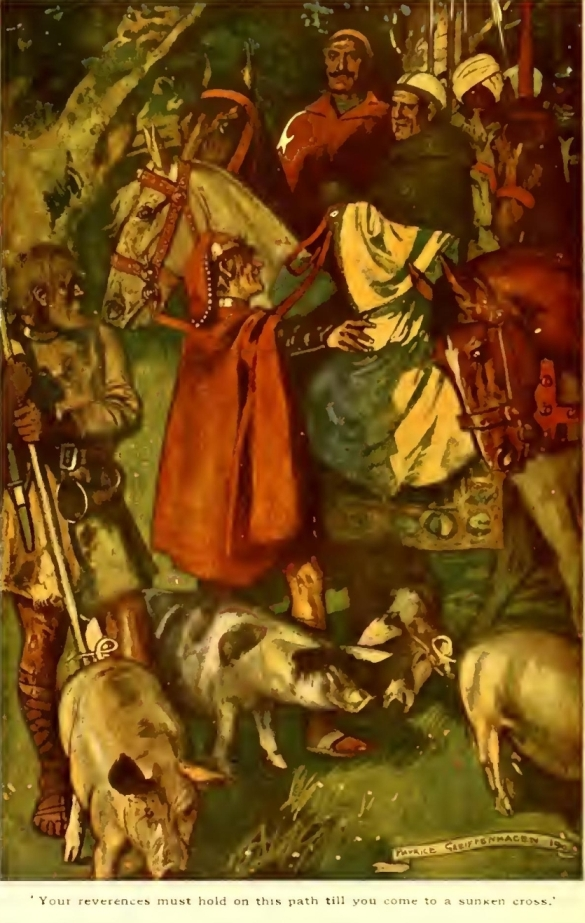
\includegraphics[height=.9\textheight]{ivanhoe/0010m}
    \caption{``Your reverences must hold on this path till you come to
    a sunken cross.''}
\end{figure}

The Abbot thanked his sage adviser; and the cavalcade, setting spurs to
their horses, rode on as men do who wish to reach their inn before the
bursting of a night-storm. As their horses' hoofs died away, Gurth said
to his companion, ``If they follow thy wise direction, the reverend
fathers will hardly reach Rotherwood this night.''

``No,'' said the Jester, grinning, ``but they may reach Sheffield if
they have good luck, and that is as fit a place for them. I am not so
bad a woodsman as to show the dog where the deer lies, if I have no mind
he should chase him.''

``Thou art right,'' said Gurth; ``it were ill that Aymer saw the Lady
Rowena; and it were worse, it may be, for Cedric to quarrel, as is most
likely he would, with this military monk. But, like good servants let us
hear and see, and say nothing.''

We return to the riders, who had soon left the bondsmen far behind them,
and who maintained the following conversation in the Norman-French
language, usually employed by the superior classes, with the exception
of the few who were still inclined to boast their Saxon descent.

``What mean these fellows by their capricious insolence?'' said the
Templar to the Benedictine, ``and why did you prevent me from chastising
it?''

``Marry, brother Brian,'' replied the Prior, ``touching the one of them,
it were hard for me to render a reason for a fool speaking according to
his folly; and the other churl is of that savage, fierce, intractable
race, some of whom, as I have often told you, are still to be found
among the descendants of the conquered Saxons, and whose supreme
pleasure it is to testify, by all means in their power, their aversion
to their conquerors.''

``I would soon have beat him into courtesy,'' observed Brian; ``I am
accustomed to deal with such spirits: Our Turkish captives are as fierce
and intractable as Odin himself could have been; yet two months in my
household, under the management of my master of the slaves, has made
them humble, submissive, serviceable, and observant of your will. Marry,
sir, you must be aware of the poison and the dagger; for they use either
with free will when you give them the slightest opportunity.''

``Ay, but,'' answered Prior Aymer, ``every land has its own manners and
fashions; and, besides that beating this fellow could procure us no
information respecting the road to Cedric's house, it would have been
sure to have established a quarrel betwixt you and him had we found our
way thither. Remember what I told you: this wealthy franklin is proud,
fierce, jealous, and irritable, a withstander of the nobility, and even
of his neighbors, Reginald Front-de-Boeuf and Philip Malvoisin, who are
no babies to strive with. He stands up sternly for the privileges of his
race, and is so proud of his uninterrupted descend from Hereward, a
renowned champion of the Heptarchy, that he is universally called Cedric
the Saxon; and makes a boast of his belonging to a people from whom many
others endeaver to hide their descent, lest they should encounter a
share of the `vae victis,' or severities imposed upon the vanquished.''

``Prior Aymer,'' said the Templar, ``you are a man of gallantry, learned
in the study of beauty, and as expert as a troubadour in all matters
concerning the `arrets' of love; but I shall expect much beauty in this
celebrated Rowena to counterbalance the self-denial and forbearance
which I must exert if I am to court the favor of such a seditious churl
as you have described her father Cedric.''

``Cedric is not her father,'' replied the Prior, ``and is but of remote
relation: she is descended from higher blood than even he pretends to,
and is but distantly connected with him by birth. Her guardian, however,
he is, self-constituted as I believe; but his ward is as dear to him as
if she were his own child. Of her beauty you shall soon be judge; and if
the purity of her complexion, and the majestic, yet soft expression of a
mild blue eye, do not chase from your memory the black-tressed girls of
Palestine, ay, or the houris of old Mahound's paradise, I am an infidel,
and no true son of the church.''

``Should your boasted beauty,'' said the Templar, ``be weighed in the
balance and found wanting, you know our wager?''

``My gold collar,'' answered the Prior, ``against ten butts of Chian
wine;--they are mine as securely as if they were already in the convent
vaults, under the key of old Dennis the cellarer.''

``And I am myself to be judge,'' said the Templar, ``and am only to be
convicted on my own admission, that I have seen no maiden so beautiful
since Pentecost was a twelvemonth. Ran it not so?--Prior, your collar is
in danger; I will wear it over my gorget in the lists of
Ashby-de-la-Zouche.''

``Win it fairly,'' said the Prior, ``and wear it as ye will; I will
trust your giving true response, on your word as a knight and as a
churchman. Yet, brother, take my advice, and file your tongue to a
little more courtesy than your habits of predominating over infidel
captives and Eastern bondsmen have accustomed you. Cedric the Saxon, if
offended,--and he is noway slack in taking offence,--is a man who,
without respect to your knighthood, my high office, or the sanctity of
either, would clear his house of us, and send us to lodge with the
larks, though the hour were midnight. And be careful how you look on
Rowena, whom he cherishes with the most jealous care; an he take the
least alarm in that quarter we are but lost men. It is said he banished
his only son from his family for lifting his eyes in the way of
affection towards this beauty, who may be worshipped, it seems, at a
distance, but is not to be approached with other thoughts than such as
we bring to the shrine of the Blessed Virgin.''

``Well, you have said enough,'' answered the Templar; ``I will for a
night put on the needful restraint, and deport me as meekly as a maiden;
but as for the fear of his expelling us by violence, myself and squires,
with Hamet and Abdalla, will warrant you against that disgrace. Doubt
not that we shall be strong enough to make good our quarters.''

``We must not let it come so far,'' answered the Prior; ``but here is
the clown's sunken cross, and the night is so dark that we can hardly
see which of the roads we are to follow. He bid us turn, I think to the
left.''

``To the right,'' said Brian, ``to the best of my remembrance.''

``To the left, certainly, the left; I remember his pointing with his
wooden sword.''

``Ay, but he held his sword in his left hand, and so pointed across his
body with it,'' said the Templar.

Each maintained his opinion with sufficient obstinacy, as is usual in
all such cases; the attendants were appealed to, but they had not been
near enough to hear Wamba's directions. At length Brian remarked, what
had at first escaped him in the twilight; ``Here is some one either
asleep, or lying dead at the foot of this cross--Hugo, stir him with the
butt-end of thy lance.''

This was no sooner done than the figure arose, exclaiming in good
French, ``Whosoever thou art, it is discourteous in you to disturb my
thoughts.''

``We did but wish to ask you,'' said the Prior, ``the road to
Rotherwood, the abode of Cedric the Saxon.''

``I myself am bound thither,'' replied the stranger; ``and if I had a
horse, I would be your guide, for the way is somewhat intricate, though
perfectly well known to me.''

``Thou shalt have both thanks and reward, my friend,'' said the Prior,
``if thou wilt bring us to Cedric's in safety.''

And he caused one of his attendants to mount his own led horse, and give
that upon which he had hitherto ridden to the stranger, who was to serve
for a guide.

Their conductor pursued an opposite road from that which Wamba had
recommended, for the purpose of misleading them. The path soon led
deeper into the woodland, and crossed more than one brook, the approach
to which was rendered perilous by the marshes through which it flowed;
but the stranger seemed to know, as if by instinct, the soundest ground
and the safest points of passage; and by dint of caution and attention,
brought the party safely into a wilder avenue than any they had yet
seen; and, pointing to a large low irregular building at the upper
extremity, he said to the Prior, ``Yonder is Rotherwood, the dwelling of
Cedric the Saxon.''

This was a joyful intimation to Aymer, whose nerves were none of the
strongest, and who had suffered such agitation and alarm in the course
of passing through the dangerous bogs, that he had not yet had the
curiosity to ask his guide a single question. Finding himself now at his
ease and near shelter, his curiosity began to awake, and he demanded of
the guide who and what he was.

``A Palmer, just returned from the Holy Land,'' was the answer.

``You had better have tarried there to fight for the recovery of the
Holy Sepulchre,'' said the Templar.

``True, Reverend Sir Knight,'' answered the Palmer, to whom the
appearance of the Templar seemed perfectly familiar; ``but when those
who are under oath to recover the holy city, are found travelling at
such a distance from the scene of their duties, can you wonder that a
peaceful peasant like me should decline the task which they have
abandoned?''

The Templar would have made an angry reply, but was interrupted by the
Prior, who again expressed his astonishment, that their guide, after
such long absence, should be so perfectly acquainted with the passes of
the forest.

``I was born a native of these parts,'' answered their guide, and as he
made the reply they stood before the mansion of Cedric;--a low irregular
building, containing several court-yards or enclosures, extending over a
considerable space of ground, and which, though its size argued the
inhabitant to be a person of wealth, differed entirely from the tall,
turretted, and castellated buildings in which the Norman nobility
resided, and which had become the universal style of architecture
throughout England.

Rotherwood was not, however, without defences; no habitation, in that
disturbed period, could have been so, without the risk of being
plundered and burnt before the next morning. A deep fosse, or ditch, was
drawn round the whole building, and filled with water from a
neighbouring stream. A double stockade, or palisade, composed of pointed
beams, which the adjacent forest supplied, defended the outer and inner
bank of the trench. There was an entrance from the west through the
outer stockade, which communicated by a drawbridge, with a similar
opening in the interior defences. Some precautions had been taken to
place those entrances under the protection of projecting angles, by
which they might be flanked in case of need by archers or slingers.

Before this entrance the Templar wound his horn loudly; for the rain,
which had long threatened, began now to descend with great violence.
